\documentclass[12pt]{article}

\title{Convergence in adaptation after domestication in the grasses}
\author{Woodhouse, M.R. and M. B. Hufford}

\usepackage[utf8]{inputenc}
\usepackage{colortbl}
\usepackage[letterpaper, margin=1in]{geometry} %package that allows changes in margins and header/footers
\usepackage{authblk}%allows footnote format for authors
\usepackage{rotating}
\usepackage{amsmath}
\usepackage{array}
\usepackage{booktabs}
\usepackage[x11names,dvipsnames,table]{xcolor}
\usepackage{tabularx}
\usepackage{mathptmx}       % selects Times Roman as basic font
\usepackage{helvet}         % selects Helvetica as sans-serif font
\usepackage{courier}        % selects Courier as typewriter font
\usepackage{type1cm}        % activate if the above 3 fonts are
                            % not available on your system
%
\usepackage{natbib}
\usepackage{makeidx}         % allows index generation
\usepackage{graphicx}        % standard LaTeX graphics tool
                             % when including figure files
\usepackage{multicol}        % used for the two-column index
\usepackage[bottom]{footmisc}% places footnotes at page bottom
\usepackage{setspace}
\usepackage{gensymb}
\usepackage{color}
\usepackage[textsize=tiny,colorinlistoftodos]{todonotes} % comments in margins

\definecolor{cornflowerblue}{rgb}{0.39, 0.58, 0.93}
\newcolumntype{G}[1]{>{\raggedright\let\newline\\\arraybackslash\hspace{0pt}}m{#1}}
\newcolumntype{C}[1]{>{\centering\let\newline\\\arraybackslash\hspace{0pt}}m{#1}}
\newcommand{\mbh}[1]{\textcolor{red}{\normalsize  #1}}
\newcommand{\mw}[1]{\textcolor{cornflowerblue}{\normalsize #1}}

\begin{document}
\maketitle

\begin{abstract}
The selection of desirable traits in crops during domestication has been well studied. In this review, the authors explore the current research to determine to what extent domestication in grass cereal crops has shaped environmental adaptation, and whether it is possible to predict which loci in a cereal might confer adaptive properties.
\end{abstract}

\section*{Introduction}
Most societies across the globe rely on domesticated crop species for survival.
Considering crop production as a measure of consumption, in 2016 alone the United States produced 384 million tons of maize, China produced 211 million tons of rice \mbh{wheat seems like a strange choice for China...why not rice?--FIXED MW}, and Nigeria produced 6.9 million tons of sorghum http://www.fao.org.
Crop physiology has changed dramatically during domestication; in the last 10,000 or so years, crops have been continually selected by humans for traits including nutrition, yield, and other attractive features.
As such, domesticated crops are often radically different from their wild relatives.

The process of domestication, wherein desirable traits in a wild species are selected for and bred by humans, is ultimately the product of genetic selection \citep{Doebley2006}.
By selectively breeding individuals in, say, a maize population that have larger ears than their parental population, one is also selecting for alleles that genetically code for the creation of larger ears. 
Notably, there are certain traits that distinguish domesticated crops from their wild progenitors \mbh{feels a little redundant to previous paragraph, though the traits mentioned here are more classic domestication syndrome traits--I yes this is focusing specifically on Domestication syndrome traits MW}, even among distantly related crops such as maize and sunflower; these traits include apical dominance or lack of branching, loss of seed dormancy, loss of bitterness, larger fruits or grains, and loss of shattering or seed dispersal (Table \ref{tab:DomTraits}).
This suite of shared traits is known as the domestication syndrome \citep{Hammer1984}.

\begin{table}
\rowcolors{2}{gray!25}{white}
\begin{center}
\caption{Prevalence of Domestication Syndrome Traits} \label{tab:DomTraits}
\begin{tabular}{p{5cm}cccl}\\\toprule  
{\bf Domestication Trait} & {\bf In Grass Crops} & {\bf In non-Grass Crops} &	{\bf References} \\\toprule
Compact plant growth & yes & yes & \citep{Gepts2010, Lenser2013}\\
Reduced axillary branching & yes & yes & \citep{Lenser2013}\\
Reduced seed dormancy & yes & yes & \citep{Gepts2010, FernndezMarn2014}\\
Changes in flowering time & yes & yes & \citep{Lenser2013}\\
Uniform flowering or maturation time & yes & yes & \citep{Lenser2013}\\
Vernalization & yes & yes & \citep{Blackman2016}\\
Increased resource allocation to harvested organ/larger organ (fruit, grain, root) & yes & yes & \citep{Miller2011}\\
Compact inforescence & yes & yes & \citep{Gepts2010, Greenwood2017}\\
Non-shattering/indehiscent fruit or grain & yes & yes & \citep{Lenser2013, Dong2014}\\
Changes in pigmentation & yes & yes & \citep{Lenser2013}\\
Self-fertilizing & yes & yes & \citep{Gepts2010}\\
Perennial to annual lifecycle  & yes & yes & \citep{Gepts2010, Miller2011}\\
Sexual to vegetative reproduction & no & yes & \citep{Lyu2017}\\
Reduced defensive structures (spines, thorns) & no & yes & \citep{Miller2011, Pickersgill2007}\\
Reduced toxicity & no & yes & \citep{Miller2011, Shlichta2018}\\
Soft or naked kernel or seed & yes & no & \citep{Wang2005}\\
Increased spikelets & yes & no & \citep{Gepts2010}\\
Increased number of kernel rows & yes & no & \citep{Lenser2013}\\\bottomrule
\end{tabular}
\end{center}
\end{table} 
 

But how can two vastly \mbh{maybe add a diverge estimate here?  How many generations between maize and sunflower?--Done MW} diverged species such as maize and sunflower  (their last common ancestor was 150 MYA \citep{Chang2004}) share the same domesticated traits? 
After all, the domestication of both maize and sunflower happened millions of years after these two species diverged.
Since these two species still share some enzymatic pathways, perhaps similar genes within these pathways have alleles that code for similar traits favored during domestication.
Shared phenotypes that are due to the modification of similar genes, or orthologs, is a phenomenon sometimes known as parallelism; parallelism is more likely to occur the more closely related any two species are \citep{Pickersgill2018}.
Conversely, it is possible for two different genes in two different enzymatic pathways in two different species to give rise to alleles which happen to code for similar traits, especially if both species experience similar selection pressures (either human or environmental).
This phenomenon is known as convergence, and in diverged species it is more likely than parallelism to result in similar phenotypic traits, since there are fewer orthologs between distantly related species.

After the initial wave of crop domestication yielded many of the aforementioned domestication syndrome traits, another level of domestication has since ensued--the adaptation of crop species to specific environments.
At both the global and the local level, distribution of crops to new environments has made it necessary for breeders to select traits that are conducive to the new environment in question.
A cultivar of maize bred to thrive at sea level, for instance, may not necessarily thrive in the colder, higher UV environment of the Andes.
Therefore, a breeder in the Andes must look for individuals in the existing domesticated maize population that are hardy under the new conditions.
However, crop adaptation faces genetic limitations that the domestication of wild progenitors never had, including loss of diversity due to genetic bottlenecks associated with both domestication and subsequent crop expansion \cite{Wang2017}. 

If domestication leads to the genetic selection of certain alleles that code for  desirable traits (such as those in the domestication syndrome), then other alleles that are conditionally neutral may be lost during domestication and expansion, particularly if the breeding population is small.
Loss of genetic diversity in a population through a genetic bottleneck can have consequences for adaptation.
For example, a dramatic genetic bottleneck "lumper" variety of potato led to the infamous Potato Famine in Ireland in the 1840s. \mbh{perhaps mention \emph{Phytopthera infestans} with a citation here?}
The Potato Famine demonstrated that by divesting a crop cultivar of its diversity, the cultivar also loses its ability to adapt to newly encountered environmental pressures, because the alleles that code for adaptive traits such as, for instance, disease resistance are lost. \mbh{Great idea to include potato famine here :-)}

The ways in which domestication has shaped the potential for adaptation in crops is the topic of this review. \mbh{I think we want to set this up more as the potential for convergence in domestication vs. adaptation due to demography (i.e., genetic bottlenecks)}
We will focus mainly on grass crops, since the major grass crop species--maize, rice, sorghum, wheat, barley, and millet--are diverged enough to allow for an analysis of trait convergence, but closely related enough to share enzymatic pathways useful in studying parallelism \mbh{before we set this up as a dichotomy, but here we argue they can occur simultaneously}.
In addition, grasses share a certain amount of genomic dynamism, including polyploidization and transposable element activity, that can give rise to new alleles which can contribute to both domestication and adaptation. \mbh{not sure I quite understand the link here to convergence, but perhaps more clear further on}
In this review we will discuss to what extent the same genes that played a role in domestication syndrome in grass crops also play a potential role in adaptation, which adaptive traits are expected to be convergent or parallel, and if it is possible to predict with any certainty which loci are likely to yield adaptive alleles.
\mbh{Let's briefly talk this through...I think we need to tweak}
\paragraph{}

\section*{Domestication in the grasses}
Grasses as a whole have been viewed by some researchers as a single genetic system \citep{pmid8379002, pmid11244100}, and there are many reasons why this point of view is useful for studying crop domestication.
The grass clade is thought to have arisen around 75 MYA \citep{BOUCHENAKKHELLADI2010, Kellogg2001} with rice, wheat, barley, millet, maize, and sorghum arising sequentially afterward (Figure \ref{fig:grassphylo}).
Prior to the radiation of the grasses, however, there was a genome duplication event approximately 70 MYA \citep{Paterson2004}, which is shared among all grass crops (Figure \ref{fig:grassphylo}), and both maize and wheat have undergone later polyploidy events after their respective species divergence (Figure \ref{fig:grassphylo}) \citep{Levy2002}.
These polyploidy events, followed by selective and ongoing fractionation, present an opportunity for grass genomes to evolve subfunctionalized homeologs; this, along with relatively high transposon activity (particularly in maize and wheat) \citep{Wicker2016, Lisch2001}, makes the grasses more susceptible to a higher rate of functional mutation compared with other crop species.  
Additionally, most grass crops were domesticated within the latitudinal boundaries of the equator and 35 N \citep{Jain1993, Gepts2010}, featuring both wet and dry seasons \citep{Jain1993}, which means that domesticated grasses shared similar environmental pressures such as temperature and day length; yet each grass cereal has been cultivated separately in separate geographic locations, including maize (Americas), sorghum (Africa), rice (Asia), millet (Eurasia), and wheat and barley (Middle East) \citep{Glmin2009}, representing approaches to domestication that take into account culturally distinct selection of favorable traits.
Taken together, these features make domesticated grass species especially conducive to a meaningful study of convergence vs parallelism in both domestication and adaptation of crops, and therefore, the six major domesticated grass crops--maize, rice, sorghum, wheat, barley, and millet--will be the focus of this review. 

\begin{figure}[h]
    \centering
    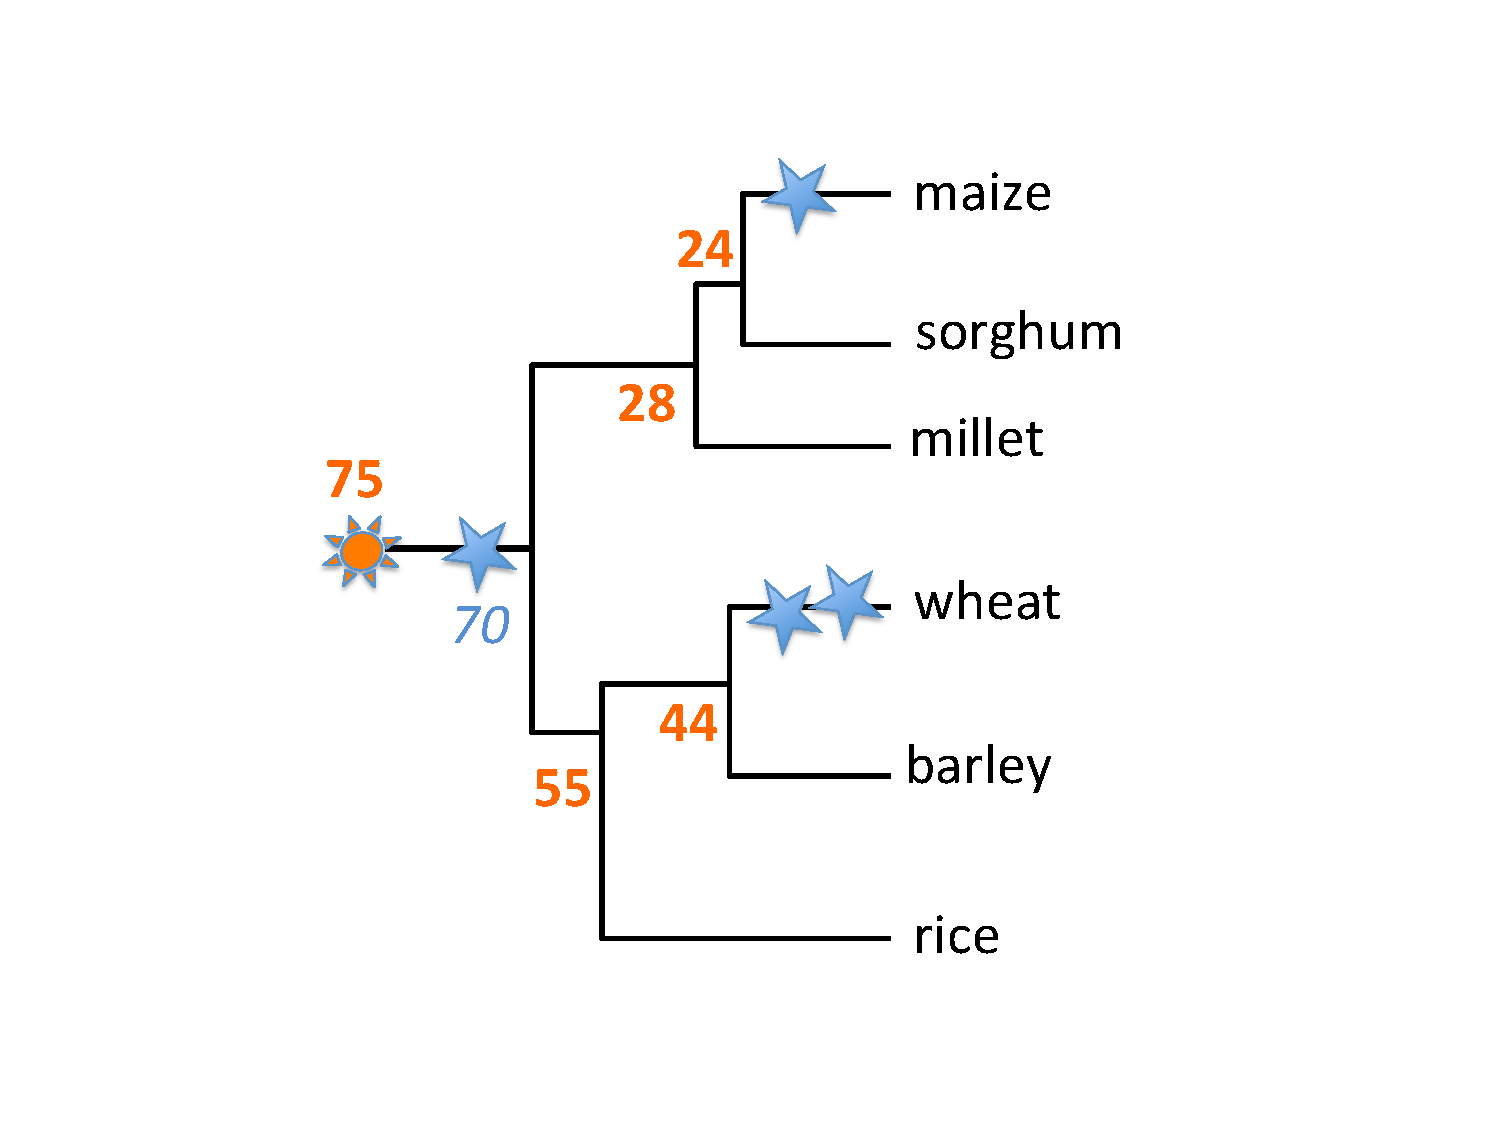
\includegraphics[width=15cm]{Figure_1.pdf}
    \caption{Simple cladogram of major cereal speciation. Numbers are in MYA (millions of years ago).
Orange sun: grass speciation event 75 MYA.  Blue stars: polyploidy events; 
the major grass polyploidy event immediately after the grass speciation event occurred 
approximately 70 MYA. The Ehrhartoideae clade, which includes rice, arose 
approximately 55MYA. The Pooideae clade, which includes wheat and barley, 
arose around 44MYA; Chloridoideae which contains foxtail millet 28 MYA, and the Panicoids, 
which include maize and sorghum, arose approximately 24MYA. The branch length is not 
proportional to the number of substitutions per site.
}
    \label{fig:grassphylo}
\end{figure}

Grass crops share a number of domestication syndrome traits observed in other non-grass crop species; these traits are summarized in the introduction and in Table 1.
However, there are a few domestication syndrome traits that are not observed in grass crops, such as reduced toxicity, reduced defensive structures like spines and thorns--by and large the wild relatives of grass crops did not have these defense mechanisms to begin with--or vegetative reproduction.
Alternately, there are some domestication syndrome traits in the grasses that are not observed in non-grass crops, such as increased spikelet number and increased number of kernel rows, because these traits occur on structures that do not exist in non-grass crop species.  

Some of the genes involved in the domestication syndrome, both within and outside of the grasses, have been identified; these genes are summarized in Table \ref{tab:Ortho} (modified from \citep{Lenser2013}).
These domestication genes are categorized in Column 3 by whether or not they have orthologs strictly within a species, orthologs across the grasses, orthologs within and outside of the grasses, or orthologs entirely outside of the grasses.
While there has been much debate regarding the delineation of parallel versus convergent traits \mbh{perhaps cite the Arendt and Reznick paper here}, for the purposes of this review we will use the definitions of both as set out in the introduction, where parallelism is defined as similar phenotypes due to mutations in orthologous genes, whereas convergence is due to mutations in genes that are not orthologous.
Column 7 in Table \ref{tab:Ortho} indicates whether a domestication gene is expected to be convergent or parallel, based on the phylogeny of orthology; for example, if a domestication gene is found only within a species, it cannot be selected in parallel.
For instance, coloration in blood orange due to selection on the Ruby gene and coloration in grapevine due to selection on the \textit{VvMYBA1-3} gene are predicted to be convergent since the alleles for these traits seem to be species-specific.
And yet there are other coloration genes, such as \textit{BADH2} and \textit{DFR}, which occur in species as diverse as rice and soybean, or rice and potato, respectively. \mbh{have they been implicated as targets of selection during domestication?}
It should be noted, however, that coloration is a very generic term, and enters into yet another level of argument regarding convergence or parallelism, associated with the physiological location of a domestication trait.
Can a trait that is observed in vastly different organs such as a potato tuber and a rice grain (as with \textit{DFR} coloration) truly be considered parallel, even if the alleles that code for them are on orthologous genes? \mbh{perhaps thinking about this as coloration of harvested plant part}
For the purposes of this review, we will keep our definitions of convergence and parallelism to within gene families and enzymatic pathways. 

\begin{sidewaystable}
\rowcolors{2}{gray!25}{white}
\begin{center}
\caption{Parallel or Convergent Orthologies} \label{tab:Ortho}
        \fontsize{7}{8}\selectfont 
    \begin{tabular}{G{3.5cm}G{2.5cm}C{3.10cm}C{3.5cm}C{1.95cm}G{2.0cm}G{1.8cm}G{1.5cm}G{1.5cm}}
\\\toprule  
{\bf Crop species} & {\bf Ortholog phylogeny} & {\bf Phylogeny of domestication trait} & {\bf Orthologous gene(s)} & {\bf Gene product} & {\bf Phenotypic trait} & {\bf Trait type} & {\bf Convergence} & {\bf References} \\\toprule
Rice, barley & Family & grass-wide & OsGA20ox-2, HvGA20ox-2 & Metabolic enzyme & Dwarfism & domestication & parallel & \citep{Asano2007, Asano2011, Jia2009}\\
Wheat & Species & species-specific, grass & Rht-1 & SH2-TF & Dwarfism & domestication & convergent & \citep{Doebley2006}\\
Sorghum, pearl millet & Family & grass-wide & dw3, d2 & Transporter protein & Dwarfism & domestication & parallel & \citep{Multani2003,Parvathaneni2013}\\
Tomato, soybean, common bean & Family/above family & outside the grasses & SP, Dt1, PvTFL1y & Signaling protein & Determinate growth & domestication & parallel & \citep{Doebley2006, Repinski2012, Liu2010, Kwak2012, Tian2010}\\
Barley, pea, strawberry & Above family & grasses and beyond & HvCEN, PsTFL1c, FvTFL1 & Signaling protein & Flowering time & both & parallel & \citep{Comadran2012, Foucher2003, Koskela2012}\\
Barley, wheat, ryegrass & Species/family & grass-wide & VRN1, BM5, TmAP1, WAP1, LpVRN1 & MADS domain TF & Flowering time & both & parallel & \citep{Asp2011}\\
Barley, wheat, maize & Species/family & grass-wide & VRN2, ZCCT1, ZmZCCT9 & Zinc finger–CCT domain TF & Flowering time & both & parallel & \citep{Huang2017}\\
Rice, barley, wheat, sorghum, sugar beet & Species/family/above family & grasses and beyond & OsPRR37, Ppd-H1, Ppd1, SbPRR37, BvBTC1 & Circadian clock pathway & Flowering time & both & parallel & \citep{MURAKAMI2005, Turner2005, Jones2008, Beales2007, Wilhelm2008, Daz2012}\\
Turnip, Brassica oleracea & Family & outside the grasses & BrFLC2, BoFLC2 & MADS domain TF & Flowering time & both & parallel & \citep{Wu2012, Yuan2009, Okazaki2006}\\
Rice, barley, pea, lentil & Family/above family & grasses and beyond & Hd17, EAM8, Mat-a, HR, LcELF3 & Circadian clock pathway & Flowering time & both & parallel & \citep{Weller2012, Matsubara2012, Zakhrabekova2012, Faure2012}\\
Rice, wheat, sunflower, barley & Family/above family & grasses and beyond & Hd3a (Heading date 3a), VRN3/TaFT, HaFT1, HvFT & Signaling protein & Flowering time & both & parallel & \citep{Yan2006, Takahashi2009, Blackman2010}\\
Rice & Species & species-specific, grass & Hd1 & Zinc finger TF & Flowering time & both & convergent & \citep{Martin2013}\\
Sorghum, rice, maize & Family & grass-wide & Sh1, OsSh1, ZmSh1 & YABBY-like TF & Shatter resistance & domestication & parallel & \citep{Lin2012}\\
Rice, wheat, maize, foxtail millet, barley, amaranth, sorghum, broomMaize millet & Species/family/above family & grasses and beyond & GBSSI, Waxy & Metabolic enzyme & Glutinous seeds & domestication & parallel & \cite{Jeon2010, Fan2008, Kawahigashi2013, Kawase2005, Hunt2012, Park2011}\\
Rice, soybean & Species/family & grasses and beyond & BADH2, GmBADH2 & Metabolic enzyme & Fragrance & domestication & parallel & \citep{Kovach2009, Juwattanasomran2010}\\
Rice, potato & Species/above family & grasses and beyond & Rd/DFR, DFR & Metabolic enzyme & Coloration & both & parallel & \citep{Furukawa2006, Zhang2009}\\
Blood orange & Species & species-specific, outside grasses & Ruby & MYB-TF & Coloration & both & convergent & \citep{Butelli2012}\\
Rice & Species & species-specific, grass & Bh4 & Transporter protein & Coloration & both & convergent & \citep{Zhu2011}\\
Soybean & Species & species-specific, outside grasses & R & MYB-TF & Coloration & both & convergent & \citep{Gillman2011}\\
Pea, potato & Above family & outside the grasses & flavonoid 3',5'-hydroxylase & Metabolic enzyme & Coloration & both & parallel & \citep{Martin2013}\\
Rice & Species & species-specific, grass & Rc & bHLH-TF & Coloration & both & convergent & \citep{Martin2013}\\
Grapevine & Species & species-specific, outside grasses & VvMYBA1-3 & MYB-TF & Coloration & both & convergent & \citep{Martin2013}\\
Maize, pearl millet, barley & Family & grass-wide & tb1, Pgtb1, INT-C & TCP-TF & Plant architecture & both & parallel & \citep{Studer2011, Remigereau2011, Ramsay2011}\\
Barley & Species & species-specific, grass & VRS1 & Homeodomain-TF & Plant architecture & both & convergent & \citep{Martin2013}\\
Maize & Species & species-specific, grass & Opaque2 & bZIP-TF & Grain quality & domestication & convergent & \citep{Martin2013}\\
Wheat, rye & Family & grass-wide & TaALMT1, ScALMT1 & Transporter protein & Metal tolerance & adaptation & parallel & \citep{Martin2013}\\
Sorghum, Maize & Family & grass-wide & SbMATE1, ZmMATE1 & Transporter protein & Metal tolerance & adaptation & parallel & \citep{Martin2013}\\
Maize, Arabidopsis & Above family & grasses and beyond & ZmVPP1, AVP1 & Vacuolar-type H(+) pyrophosphatase & Drought tolerance & adaptation & parallel & \citep{Wang2016}\\
Rice & Species & species-specific, grass & OsAHL1 & AT-hook PPC domain & Drought tolerance & adaptation & convergent & \citep{Zhou2016}\\
Barley, wheat & Family & grass-wide & HVA1, Wrab18, Wrab19 & LEA protein & Cold tolerance & adaptation & parallel & \citep{Hong1988, pmid16755132}\\
Wheat, barley & Family & grass-wide & Wcs19, Wcor14, Wcor15, Bcor14b & Cor protein & Cold tolerance & adaptation & parallel & \citep{Takumi2003}\\
Barley, maize, spinach & Above family & grasses and beyond & HvPIP2;1, ZmPIP2-4, PM28A & Aquaporin & Soil salinity & adaptation & parallel & \citep{Katsuhara2002, Zhu2005, Fotiadis2000}\\
Rice, foxtail millet, tomato & Above family & grasses and beyond & OsASR1, OsASR3, SiASR1, SlASR1 & ABA stress ASR protein & Soil salinity & adaptation & parallel & \citep{Li2017, Konrad2008}\\
Maize & Species & species-specific, grass & Rp3 & NBS-LRR & Pathogen resistance & adaptation & convergent & \citep{pmid12242248}\\
Wheat, rice, sorghum & Family & grass-wide & LR34 & ABC transporter & Pathogen resistance & adaptation & parallel & \citep{Krattinger2010}\\
\end{tabular}
\end{center}
\end{sidewaystable}

What might cause domestication syndrome traits to be parallel (i.e. orthologous) rather than convergent?
Lenser and Theissen's 2013 review \citep{Lenser2013} sets out four examples: (1) Genes occupying a nodal position upstream of genes that effect domestication traits; (2) Genes involved in simple metabolic pathways, because only a minimal set of genes serves as a potential mutational target to change a given trait (such as \textit{Waxy}, Table \ref{tab:Ortho}); (3) genes with fewer pleiotropic effects, such as the MYB genes (i.e. \textit{DFR}) associated with changes in fruit or seed color; (4) domestication-related alleles that are already present at low frequency within a wild population. 
The first three cases all rely on the retention of the orthologous genes throughout evolution that have not undergone functional divergence.
Therefore, loss of certain orthologs prior to widespread crop domestication would ensure that parallel domestication for some traits would be impossible.
Some of the genes predicted as convergent in Table \ref{tab:Ortho} could have lost their orthologs in other species over evolutionary time.

Table \ref{tab:Ortho} gives us a starting point to predict which domestication genes are likely to be found in the grasses, which genes in the grasses are likely to be parallel, and which are likely to be convergent. This is useful if we wish to breed wild grass relatives for domestication traits, or create hybrids among existing cultivars, since we can now associate favorable phenotypes and QTLs with orthologs across species by simple comparative genomics. In fact, comparative genomics can easily demonstrate that many of the genes in Table \ref{tab:Ortho} described as convergent do in fact have orthologs in other clades, even if the function of these orthologs have yet to be deduced (Figure 2).  But to what extent can this knowledge help us to understand how domestication has impacted a crop's ability to adapt to new environments?
\paragraph{}

\section*{Adaptation in the grasses}
An adaptive trait is one that interacts or responds to the environment in a way that helps an organism to thrive. For domesticated crops, however, adaptive traits that reverse desired domestication phenotypes such as yield, fragrance, flavor, or shatterproofing would not be considered favorable; therefore, we will narrow down the definition of an adaptive trait in this review to one that interacts or responds to the environment favorably but does not detract from desired domestication traits.  Perhaps it is also necessary to define what specifically is meant by "environment." A straightforward (and admittedly simplistic) way would be to break  "environment" down to discrete features, which can include: The level of carbon dioxide in the air; the level of UV radiation due to altitude; temperature; daylength; humidity; rainfall; wind; soil nutrient load; soil salinity; and pathogen microbiome.  By dividing the environment into these discrete elements, we can now address each element individually by asking what sort of adaptive trait we would expect to observe in response to each, and how many of these adaptive traits are expressed in the same genetic pathway as known domestication genes. 

If we take another look at Table \ref{tab:Ortho}, Column F, we find descriptions of domestication phenotypes that seem to also describe traits that would be involved in response to environment. For example, variation in flowering time is known to be a response to photoperiod sensitivity: the gene \textit{ZmCCT9} in maize appears to be involved in flowering under the long days of higher latitudes in the Americas, but a transposon insertion upstream of \textit{ZmCCT9} in domesticated maize cultivars is thought to have led to reduced photoperiod sensitivity, which has allowed domesticated maize to expand its range ~\citep{Huang2017}.  This is an excellent example of a domestication-related gene that has an environmentally adaptive component. 

Another example of a domestication trait with an adaptive component is coloration. Loss of coloration has been favored in a variety of cereal cultivars, from rice to maize, as a cultural preference (ref?). As it turns out, coloration assists with UV tolerance in cereals and other plant species ~\citep{pmid8058838, Gould2004}. Therefore, a return of coloration could likely lead to a greater tolerance of UV radiation in cereals that were bred at higher elevations ~\citep{Pyhjrvi2013}.  Table \ref{tab:Ortho} attempts to match examples of adaptation traits to domestication traits, where possible, using the definition of adaptive as described above. 

On the flip side, there are a number of adaptive traits unlikely to have a domestication component, since they appear unrelated to domestication syndrome traits. These include (but are not limited to) drought tolerance; cold tolerance; soil salinity; and pathogen defense.  Table \ref{tab:Ortho} includes some adaptive genes and their orthologs, and whether or not they are associated with domestication traits.  Adaptive genes not expected to be associated with domestication include the maize \textit{ZmVPP1} gene, where an upstream insertion is linked to drought tolerance ~\citep{Wang2016}.  Since this gene has a drought-tolerant ortholog in Arabidopsis, \textit{AVP1} ~\citep{Gaxiola2001}, it suggests that orthologs could exist elsewhere in the cereals as well. However, another drought-tolerance gene in rice, \textit{OsAHL1} ~\citep{Zhou2016}, does not appear to have a defined drought-tolerant ortholog in any other species at the time of this writing. Wheat and barley possess a small family of cold-tolerance genes including \textit{Wcs19} ~\citep{pmid8219063}, \textit{Wcor14} ~\citep{pmid10846621} and \textit{Bcor14b} ~\citep{pmid9952464}, all of which encode chloroplast-targeted COR proteins analogous to the Arabidopsis protein \textit{COR15a}  ~\citep{pmid9826741, Takumi2003}. The LEA protein orthologs \textit{HVA1} and \textit{Wrab 18/19} in barley and wheat, respectively, are also associated with cold tolerance ~\citep{Hong1988, pmid16755132}. Transcript and protein levels of the barley \textit{HvPIP2} aquaporin gene were found to be down-regulated in roots but up-regulated in the shoots of plants under salt stress ~\citep{Katsuhara2002}.  \textit{HvPIP2} has an ortholog in maize, \textit{ZmPIP2-4} ~\citep{Zhu2005}, and in spinach, \textit{PM28A} ~\citep{Fotiadis2000}. There are also the ASR (abscisic acid, stress, and ripening-induced) genes that are associated with salinity tolerance in rice ~\citep{Joo2013}, \textit{Setaria} (millet) ~\citep{Li2017}, and tomato ~\citep{Konrad2008}. 

Of course, finding orthologs for genes known to be adaptive is no guarantee that the function will be similar in different species. Though foxtail millet has a functional ortholog of the maize \textit{tb1} (\textit{teosinte branched1}) gene ~\citep{pmid9087405}  which restricts branching in domesticated maize, the foxtail millet ortholog only exhibits slight control over branching, which shows that even though two species might share orthology for a gene, it does not mean that the phenotype will be the same in both species ~\citep{Doust2004}. And so far, we have only discussed adaptive phenotypes that are driven by alleles in one locus; this neglects all the other adaptive phenotypes that are due to alleles at multiple loci.  Most importantly, however, the extent to which we can expect to find adaptive alleles for existing orthologs is dependent on the severity of the domestication bottleneck within a given cereal species.

Domestication bottlenecks are the result of selection for traits that make for desirable crops but not necessarily for environmental adaptability. Massive nucleotide diversity loss is reported in domesticated bread wheat ~\citep{Haudry2007}, maize (with an increase in deleterious alleles) ~\citep{pmid9539756, Wang2017}, rice ~\citep{pmid17218640}, Sorghum ~\citep{Hamblin2006}, and barley ~\citep{Kilian2006} compared with wild relatives, demonstrating that loss of diversity is widespread in cultivated grasses and is a phenomenon that is distinct from uncultivated wild relatives. These results suggest that domestication itself is responsible for the loss of diversity, and because of this, attempts to adapt domesticated grasses to new environments could pose a challenge.  

Outside of breeding to a wild relative, is it possible for cereal crops to be rescued from a diversity bottleneck? We have seen that grasses tend to have relatively active transposons, and this transposon activity may permit a higher mutation rate in cereals than in other crops, allowing for new alleles to arise in a population.  In Table \ref{tab:Ortho}, several of the domestication and adaptive phenotypes are due to a transposon insertion somewhere in the functional region of a gene: \textit{tb1} ~\citep{Studer2011}, \textit{ZmCCT9}, and \textit{ZmVVP1}, to name just a few. In addition, diversity in waxy foxtail millet crops in southeast Asia was shown to be mediated by multiple transposable element insertions ~\citep{Kawase2005}. However, a comprehensive review of TEs and plant evolution ~\citep{Lisch2001} suggests that our understanding of the role of transposable element activity in crop adaptation is largely anecdotal and might be overstated, but perhaps can be better elucidated by harnessing the recent advances in genomics such as more sophisticated TE annotation protocols, whole-genome sequencing, and comparative algorithms.  Using these advances in genome biology, a recent study by Lai and coworkers found that transposon insertions may have played an important role in creating the variation in gene regulation that enabled the rapid adaptation of domesticated maize to diverse environments ~\citep{Lai2017}. 

Loss of allelic diversity due to domestication bottlenecks may have a more significant impact on those adaptive phenotypes that are controlled by the same genes that control domestication phenotypes (such as \textit{ZmZCCT9}), rather than on the genes that appear unrelated to domestication (such as \textit{ZmVPP1}).  So it is not a foregone conclusion that a bottleneck in a flowering time allele, for instance, would necessarily lead to a bottleneck in an allele related to drought tolerance, unless loss of diversity in a population were severe and genome-wide, or unless drought tolerance and flowering time were phenotypically or genetically linked. Therefore, one might predict that selection for transposable element insertion would be greater for domestication-syndrome adaptation alleles than in adaptation alleles unrelated to domestication syndrome.  

But another way an adaptation trait could escape a domestication bottleneck is if the domestication-syndrome allele were on a gene with a retained homeolog, allowing for subfunctionalization or neofunctionalization of the other homeolog to an adaptive allele.  Neofunctionalization of homeologs is widespread in maize ~\citep{Hughes2014}, which has undergone a recent tetraploidy event approximately 5-12MYA ~\citep{Swigonova2004}; and in bread wheat, subfunctionalization of homeologs as a result of  wheat's hexaploidy event appear to have given rise to alleles associated with baking quality ~\citep{Pfeifer2014}.  

To some extent, it can be predicted which homeolog in a post-polyploid cereal is likely to be adaptive. It is known that of the two retained post-polyploidy subgenomes in maize, one undergoes less fractionation and is more highly expressed than the other (i.e. the dominant subgenome) ~\citep{Woodhouse2010, Schnable2011}, and there is evidence that fractionation is biased not only in maize, but in wheat as well ~\citep{Eckardt2014}.  Schnable and Freeling found that of the "classical" maize genes, or characterized genes that have a known mutant phenotype, the majority are on the less fractionated subgenome ~\citep{Schnable20112}. Many of these genes, such as \textit{tb1}, \textit{Waxy}, \textit{Opaque2}, and several starch synthesis and coloration genes not in Table \ref{tab:Ortho}, have a domestication syndrome phenotype in maize.  Additionally, recent work has suggested that the genes on the more highly expressed subgenome in maize contribute more to phenotypic variation than the less expressed subgenome ~\citep{RennyByfield2017} because they are under greater purifying selection.  If genes associated with domestication tend to be on the less fractionated subgenome, and greater phenotypic variation is observed in the less fractionated subgenome, then adaptive traits should more likely be associated with the homeolog on the less fractionated subgenome.  Indeed, two genes associated with adaptive phenotypes in maize from Table \ref{tab:Ortho}, \textit{ZmVPP1} (drought tolerance) and \textit{ZmPIP2-4} (soil salinity) are both found on the less fractionated subgenome ~\citep{Schnable20112}. Yet about forty percent of the genes on the more fractionated subgenome do exhibit some amount of expression dominance and phenotypic variation ~\citep{RennyByfield2017}, and genome dominance alone is not a guarantee that adaptive alleles could not arise on the more fractionated genome as well.  

Finally, there are some adaptive traits that are less likely to have orthologs in even closely related species. These include pathogen resistance and stress response. While there are examples of pathogen defense and stress response genes in the grasses that are orthologous to other species (Table \ref{tab:Ortho}), by and large, genes that code for traits involved in plant defense and stress response are frequently orphan genes, or genes that are specific to a particular lineage and share no defined orthologs with any outgroup ~\citep{Woodhouse2011}; reviewed in ~\citep{Arendsee2014}. Orphan genes tend to be very dynamic, arising and becoming lost much faster than their basal counterparts ~\citep{Freeling2008}.  If an adaptive trait such as pathogen resistance is dependent on these orphan-type genes, which quite often are unique even in individual cultivars within the same crop species, then we would not expect to see convergence of this trait at the alleleic level in cereal adaptation, since each species--indeed, each cultivar--would be expected to have its own unique, "outward-facing" suite of orphan genes that would confer environmental adaptation uniquely to its niche. Orphan genes often propagate through trans duplication ~\citep{Freeling2008, Arendsee2014}; therefore, movement of these genes to a new region whose local euchromatic status can confer novel expression patterns to the mobilized gene can be a strong source of adaptation, especially since it has been shown that stressful environments can stimulate activation of transposable elements ~\citep{Beguiristain2001, Makarevitch2015}  reviewed in ~\citep{Negi2016}, and this is one way that crop species might be able to escape domestication bottlenecks in adaptation.

\section*{Conclusions}
This review set out to explore how domestication has influenced the potential for adaptation in the grasses.  Factors of domestication that have influenced adaptation include the selection for domestication traits that also have adaptive qualities, and to what extent diversity of a locus has undergone a domestication bottleneck. We discussed the possible ways that a crop might escape a domestication bottleneck, including homeolog sub- or neofunctionalization, transposable element activity, and trans duplication or fast-evolvability of lineage-specific adaptive genes. We also set out to see whether it is possible to predict the likelihood of adaptability of any given trait, irrespective of domestication syndrome effects. How realistically we can predict this in any given cereal crop is dependent upon  (1) the existence of an ortholog to a known adaptive gene in another species; (2) the retention of functionality in the ortholog; (3)  which subgenome a putatively adaptive gene is on within a species that had undergone a recent polyploidy; and (4) the propensity of an adaptive gene or gene family to be orthologous.   Table \ref{tab:Ortho} attempts to summarize these findings by correlating adaptivity with domestication traits as well as orthology in other species.  


\bibliographystyle{plain}
\bibliography{convergence.bib}

\end{document}
This is never printed
